\newpage

\section{Design}

\begin{comment}
 What is required for the Design Section:
 - Aesthetic Prototype ( CAD Images, photos of physical prototypes, drawings )
 - Design for Manufacture, Assembly, Maintenance
 - Block Diagrams
 - Wiring Diagrams
 - State Transition Diagrams
 - Technology ( languages, hardware, etc. )
 - Simulation
 - Modeling
\end{comment}

\subsection{Aesthetic Prototype} % Neena will input the images here

Following extensive brainstorming and analysis, our team carefully evaluated a wide range of potential features and implementation strategies for our smart lock system. Ultimately, we selected the concept of using a solenoid-based locking mechanism controlled via a keypad and a smartphone app. This approach balanced feasibility, security, and user convenience. Our selection process included the use of the 6-3-5 method, which helped generate and refine a wide range of ideas across five categories: Hardware \& Mechanics, Smartphone Integration, Security Features, Software \& Control, and Advanced Features. We also brainstormed ideas of how the lock would potentially look like, for easy installation and fix up when an issue arises. All of our ideas were formed based on this appendix section: \ref{BrainstormingIdeas}.

\subsection{Design for Manufacture, Assembly, Maintenance} % we need to add more detail from our previous work from 123A...read his comments from draft
\subsubsection*{Design For Manufacture}
Our Design for Manufacture (DFM) is illustrated in Figure~\ref{fig:DFM} below.

\begin{figure}[!ht]
    \centering
    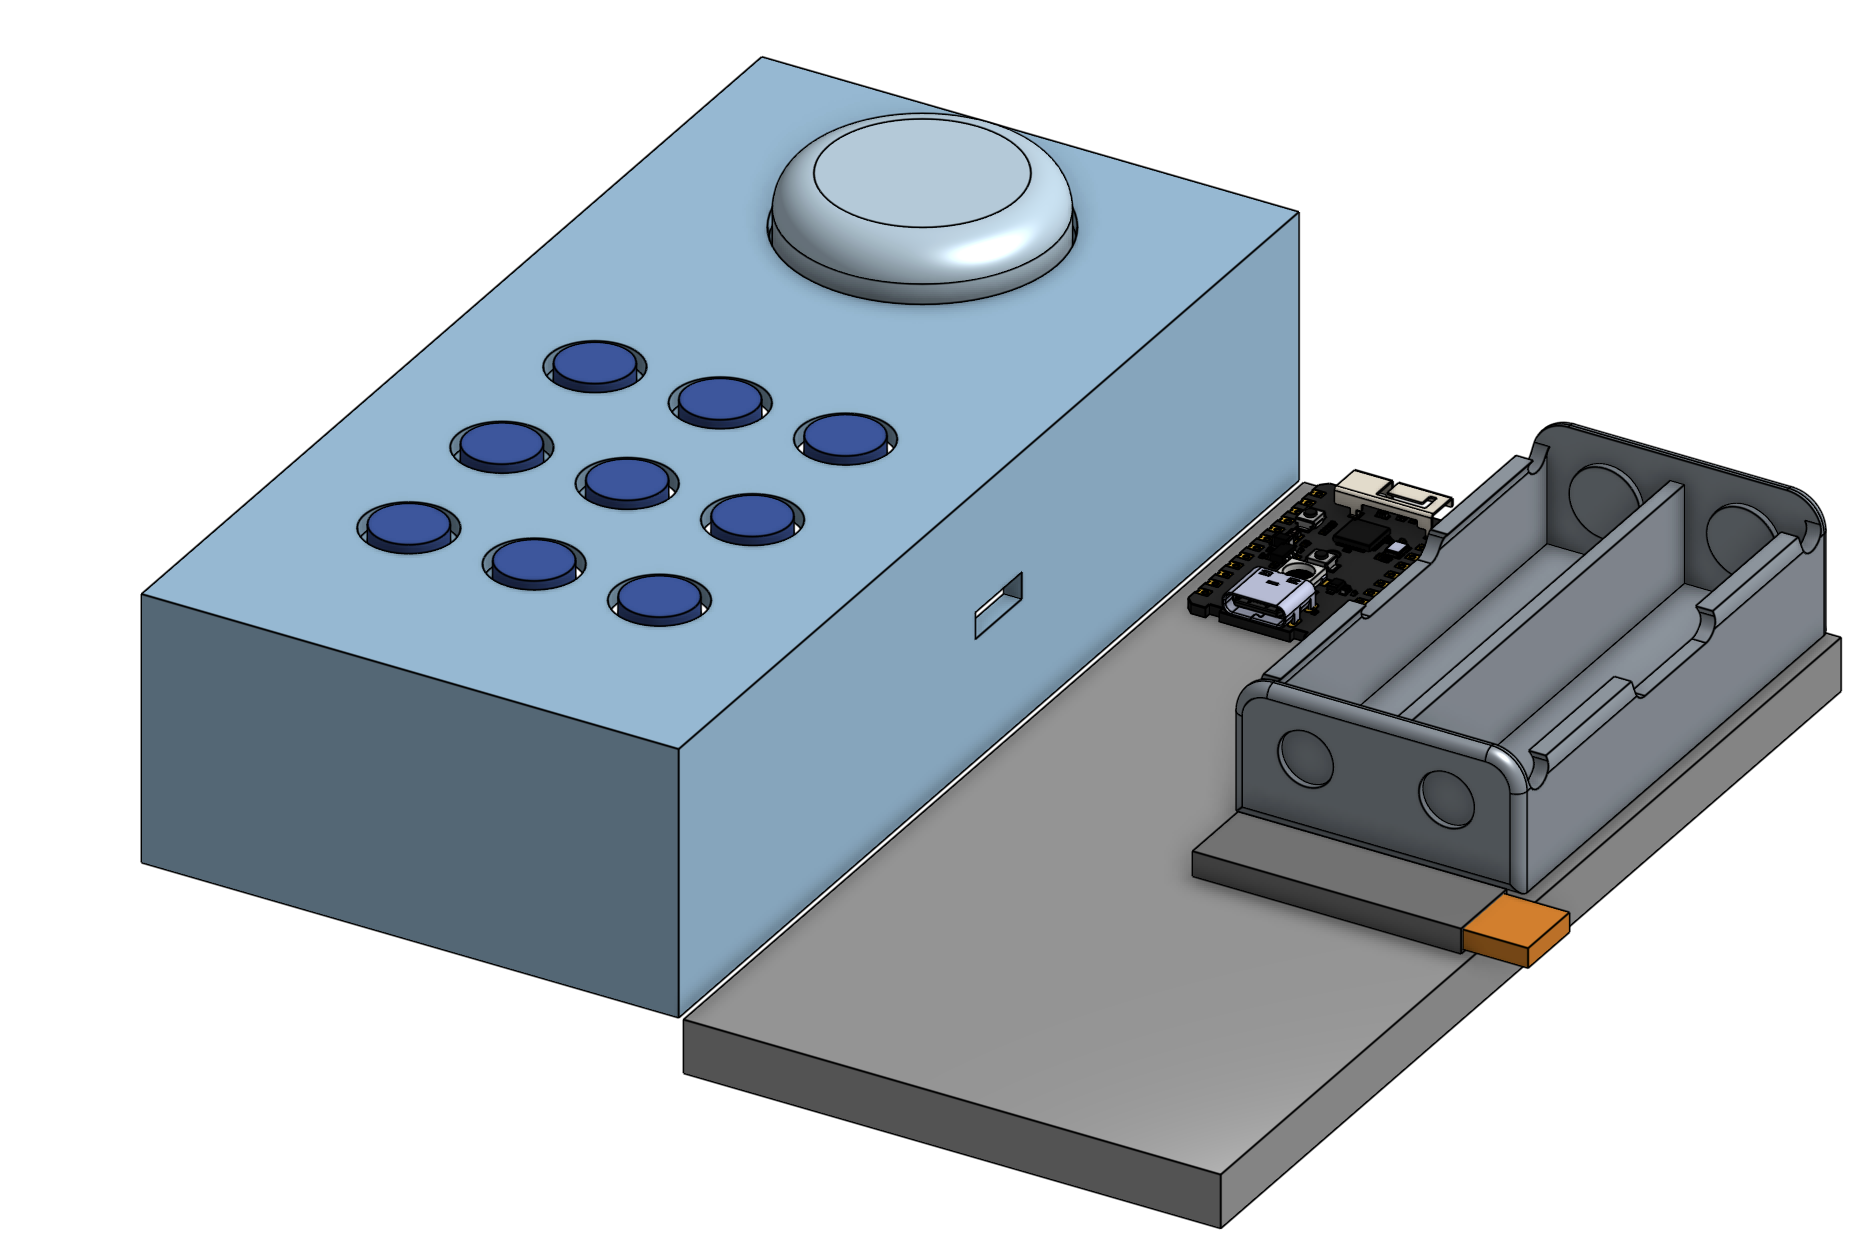
\includegraphics[width=0.80\textwidth]{img/DFM side view.png}
    \caption{DFM}
    \label{fig:DFM}
\end{figure}

As shown in the figure, the front of the device features an integrated keypad for primary user input, with space allocated for an additional module to support secondary authentication — enhancing security by verifying the identity of the user. Internally, the design houses the microcontroller, a rechargeable battery pack, and a solenoid lock mechanism.

The form factor has been developed with modern aesthetics and user-friendliness in mind, ensuring that the device is both visually appealing and intuitive for homeowners to operate. Component placement has also been optimized for efficient assembly, accessibility, and long-term maintainability.

\subsubsection*{Design For Assembly}
To ensure ease of assembly, our smart lock design emphasizes modular components, minimal fasteners, and intuitive alignment features. Figure~\ref{fig:DFA_Exploded} illustrates the exploded view of the product, showing the order and orientation of each major part during assembly.

\begin{figure}[!htbp]
    \centering
    \begin{subfigure}[b]{0.48\textwidth}
        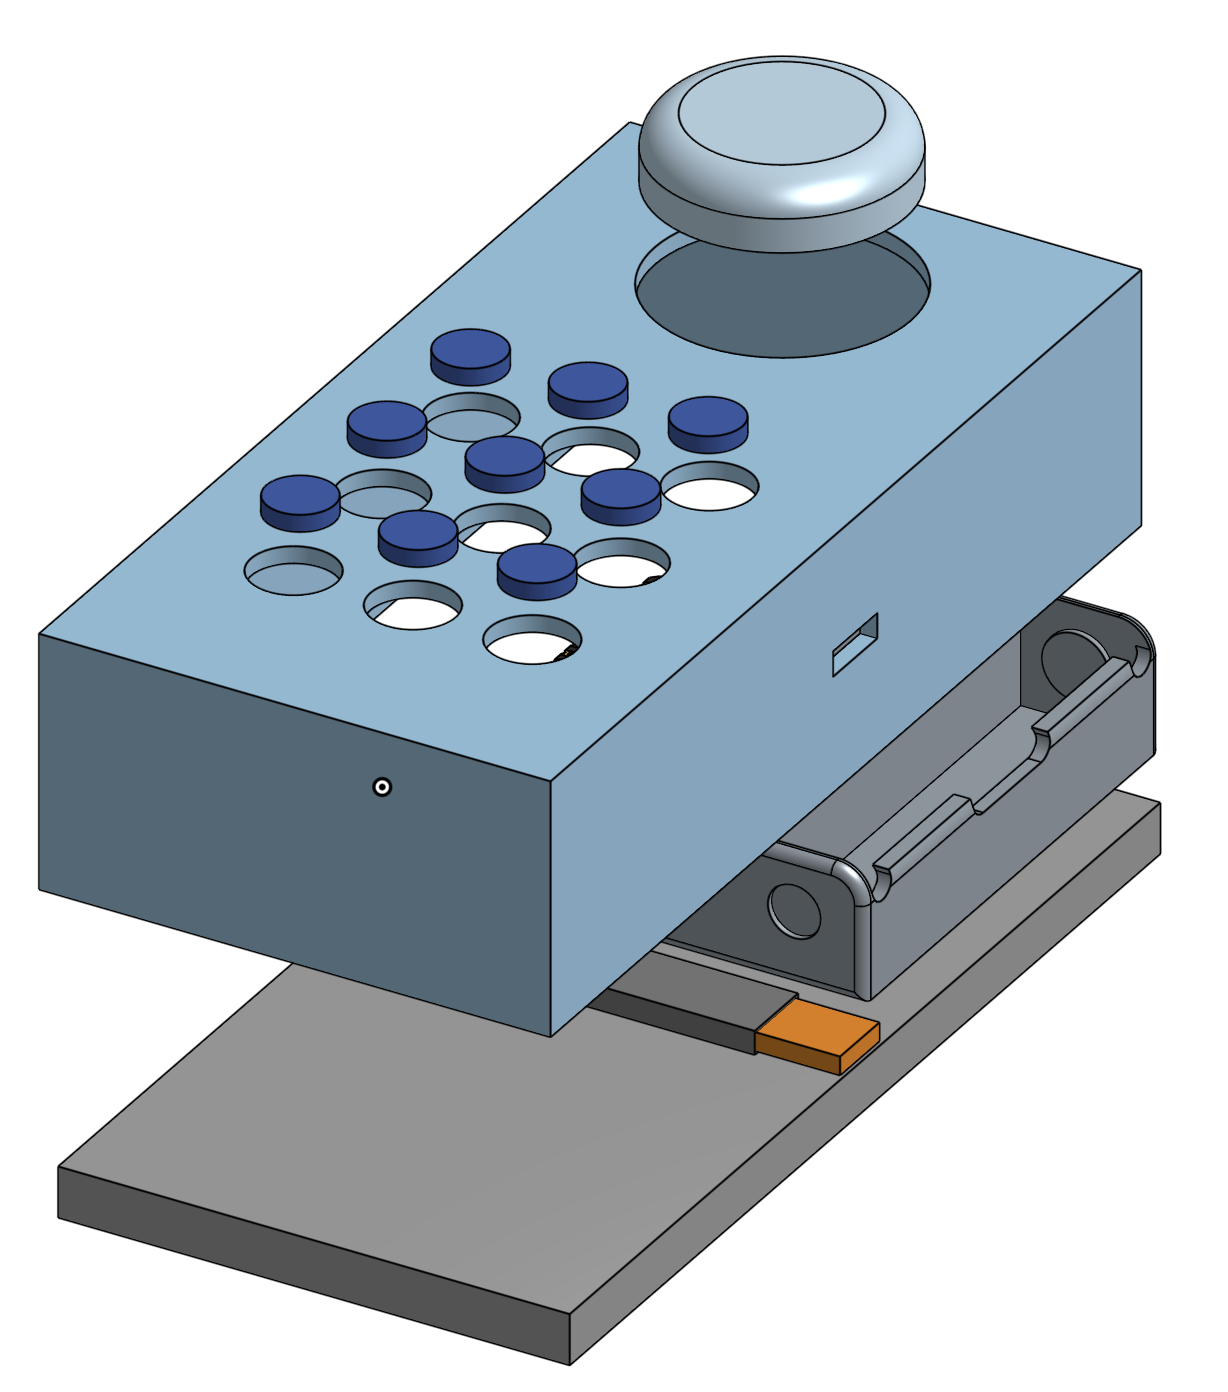
\includegraphics[width=\textwidth]{./img/DFA_Right.png}
        \caption{Exploded view right side}
        \label{fig:DFA_Right}
    \end{subfigure}
    \hfill
    \begin{subfigure}[b]{0.48\textwidth}
        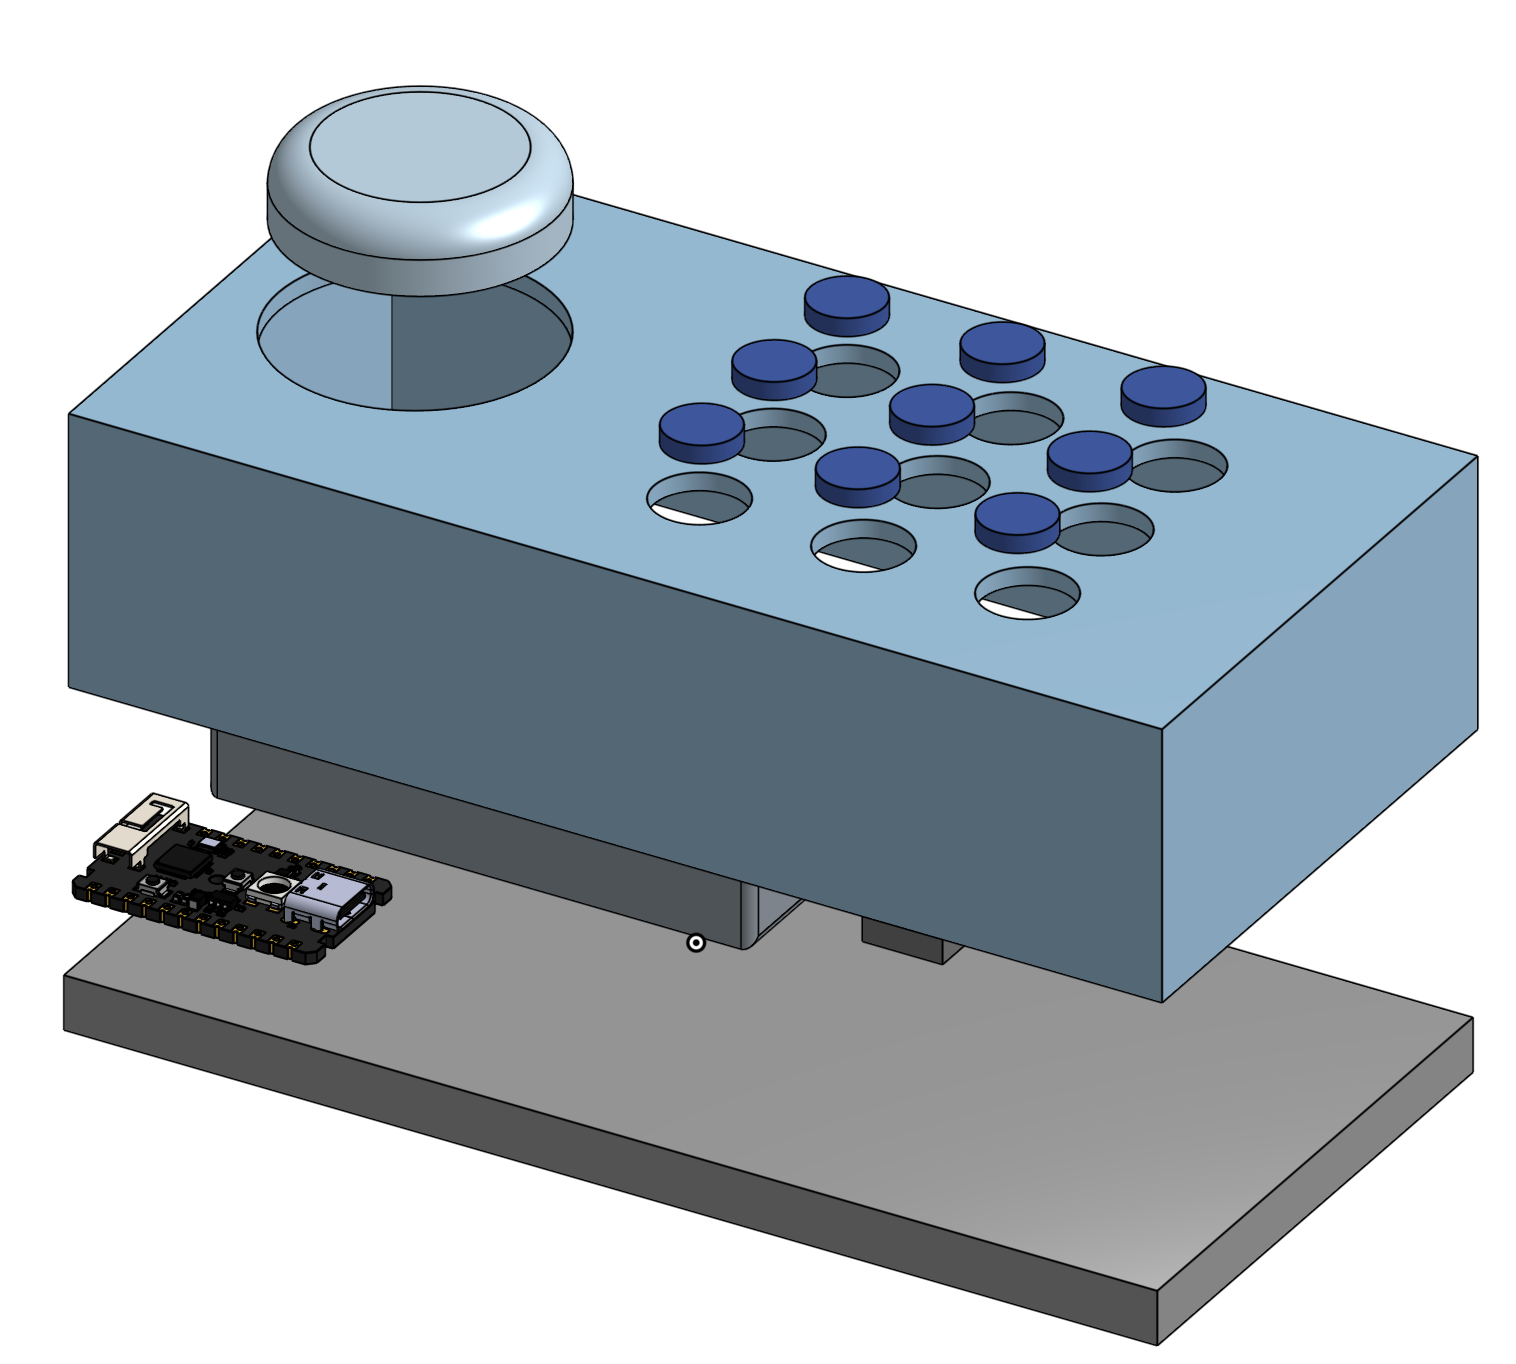
\includegraphics[width=\textwidth]{./img/DFA_Left.png}
        \caption{Exploded view left side}
        \label{fig:DFA_Left}
    \end{subfigure}
    \caption{First lock design}
    \label{fig:DFA_Exploded}
\end{figure}

The design separates the internal electronics (microcontroller, battery pack, and PCB) as a single sub-assembly that can be installed into the enclosure before final sealing. The keypad snaps into place on the front panel, and the housing is secured with four screws for quick final assembly. The overall approach minimizes assembly time and reduces the potential for user or manufacturing error.

\subsubsection*{Design for Maintenance}
The smart lock is engineered for long-term usability with minimal service requirements. A key feature of the design is the accessible battery compartment, which allows users to replace batteries without disassembling the entire unit. Standard Phillips screws secure the housing, avoiding the need for proprietary tools and simplifying field servicing.

Internally, components such as the microcontroller and solenoid lock are mounted modularly, allowing them to be replaced individually if a failure occurs. This modular approach extends the product's usable life and reduces electronic waste. Over-the-air (OTA) firmware updates are supported via the smartphone app, enabling remote bug fixes and feature updates without physical access.

Maintenance is further supported through built-in diagnostics: users receive alerts for low battery, Wi-Fi disconnection, or tampering, helping address issues before they escalate. The device is designed to operate reliably for several years with only basic battery replacement and no specialized maintenance.

\subsection{Block Diagrams}

For our block diagram, we will describe how we are going to connect our system together for our hardware, software, along with our server. The figure \ref{fig:blockDiagram} illustrates the entire system architecture. Starting from the left, we have the keypad that allows users to input access codes to control the locking mechanism. The keypad sends these inputs to the microcontroller, which acts as the central processing unit for the system.

\begin{figure}[ht]
    \centering
    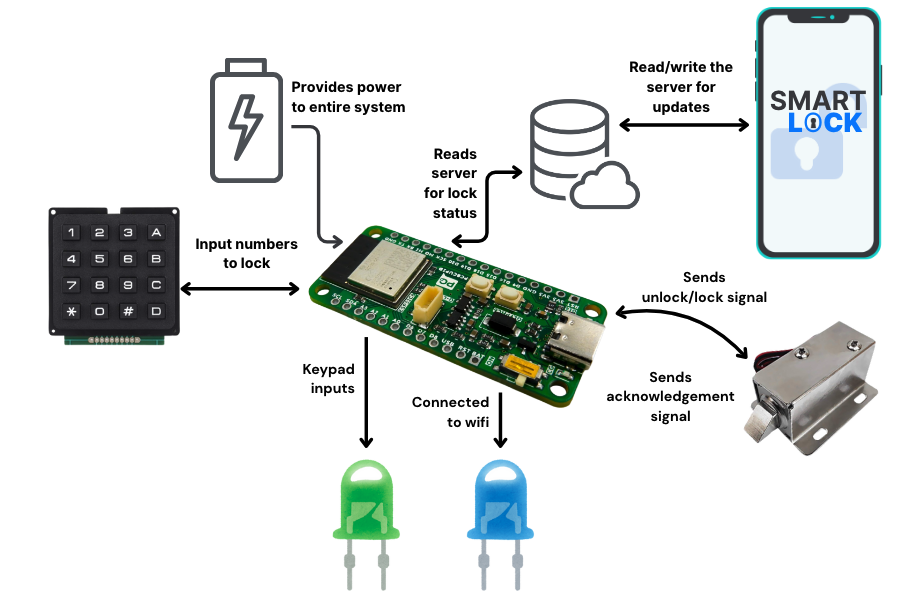
\includegraphics[width=0.80\textwidth]{img/blockDiagram.png}
    \caption{Block Diagram}
    \label{fig:blockDiagram}
\end{figure}

The microcontroller processes the user input and communicates with the solenoid lock to either engage or disengage the locking bolt based on the verification of the input code. Additionally, the microcontroller connects to the Wi-Fi module to enable remote communication with our server.

On the software side, the server hosts the backend services responsible for managing user authentication, storing access logs, and syncing lock states. It communicates with the microcontroller over the internet, allowing authorized users to control the lock remotely through a mobile application.

The mobile application serves as the user interface, enabling users to send lock or unlock commands, receive status updates, and manage access credentials. This client-server interaction ensures that users can securely control their smart lock from anywhere, while the system maintains real-time synchronization between hardware and software components.

Together, these interconnected blocks form a cohesive system that balances local authentication via the keypad with remote management through the server and mobile app, ensuring convenience and security.

\subsection{Wiring Diagrams}

In the wiring diagram shown in figure \ref{fig:wiringDiagram}, you can observe the specific pin connections between the ESP32-C3 microcontroller and the various hardware components in our system. These connections directly correspond to the GPIO (General Purpose Input/Output) pins configured in our firmware, ensuring that the software interfaces correctly with the physical devices.

\begin{figure}[ht]
    \centering
    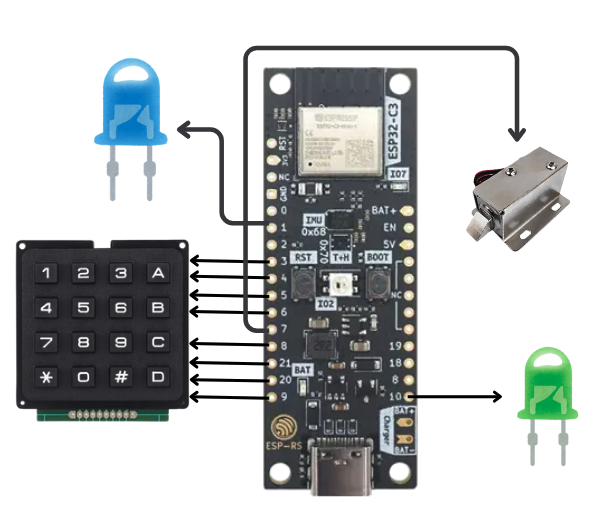
\includegraphics[width=0.80\textwidth]{img/wiringDiagram.png}
    \caption{Wiring Diagram}
    \label{fig:wiringDiagram}
\end{figure}

Starting with the keypad, each row and column line is connected to designated GPIO pins on the ESP32-C3, allowing the microcontroller to detect button presses through a matrix scanning method. This setup enables efficient reading of multiple keys with minimal pin usage. The solenoid lock control is wired to a digital output pin, which is driven high or low by the microcontroller to activate or deactivate the lock mechanism. A mosfet transistor is included in the circuit to handle the higher current required by the solenoid, protecting the ESP32-C3 from damage. Additionally, the ESP32-C3’s Wi-Fi antenna and power lines are properly connected to ensure stable wireless communication and device operation. Power supply lines are clearly marked, showing how the system components are powered, whether from an external source or regulated onboard power. The wiring diagram serves as a vital reference during assembly and troubleshooting, providing a clear mapping of all hardware interfaces. Correct adherence to this diagram ensures that the system components operate reliably and the software can control the hardware as intended.

\subsection{State Transition Diagrams}
Figure \ref{fig:stateTransitionDiagram} illustrates the state machine used in our smart lock system. This diagram outlines the various operational states of the system and the transitions between them, triggered by user inputs, system events, or remote commands.

\begin{figure}[ht]
    \centering
    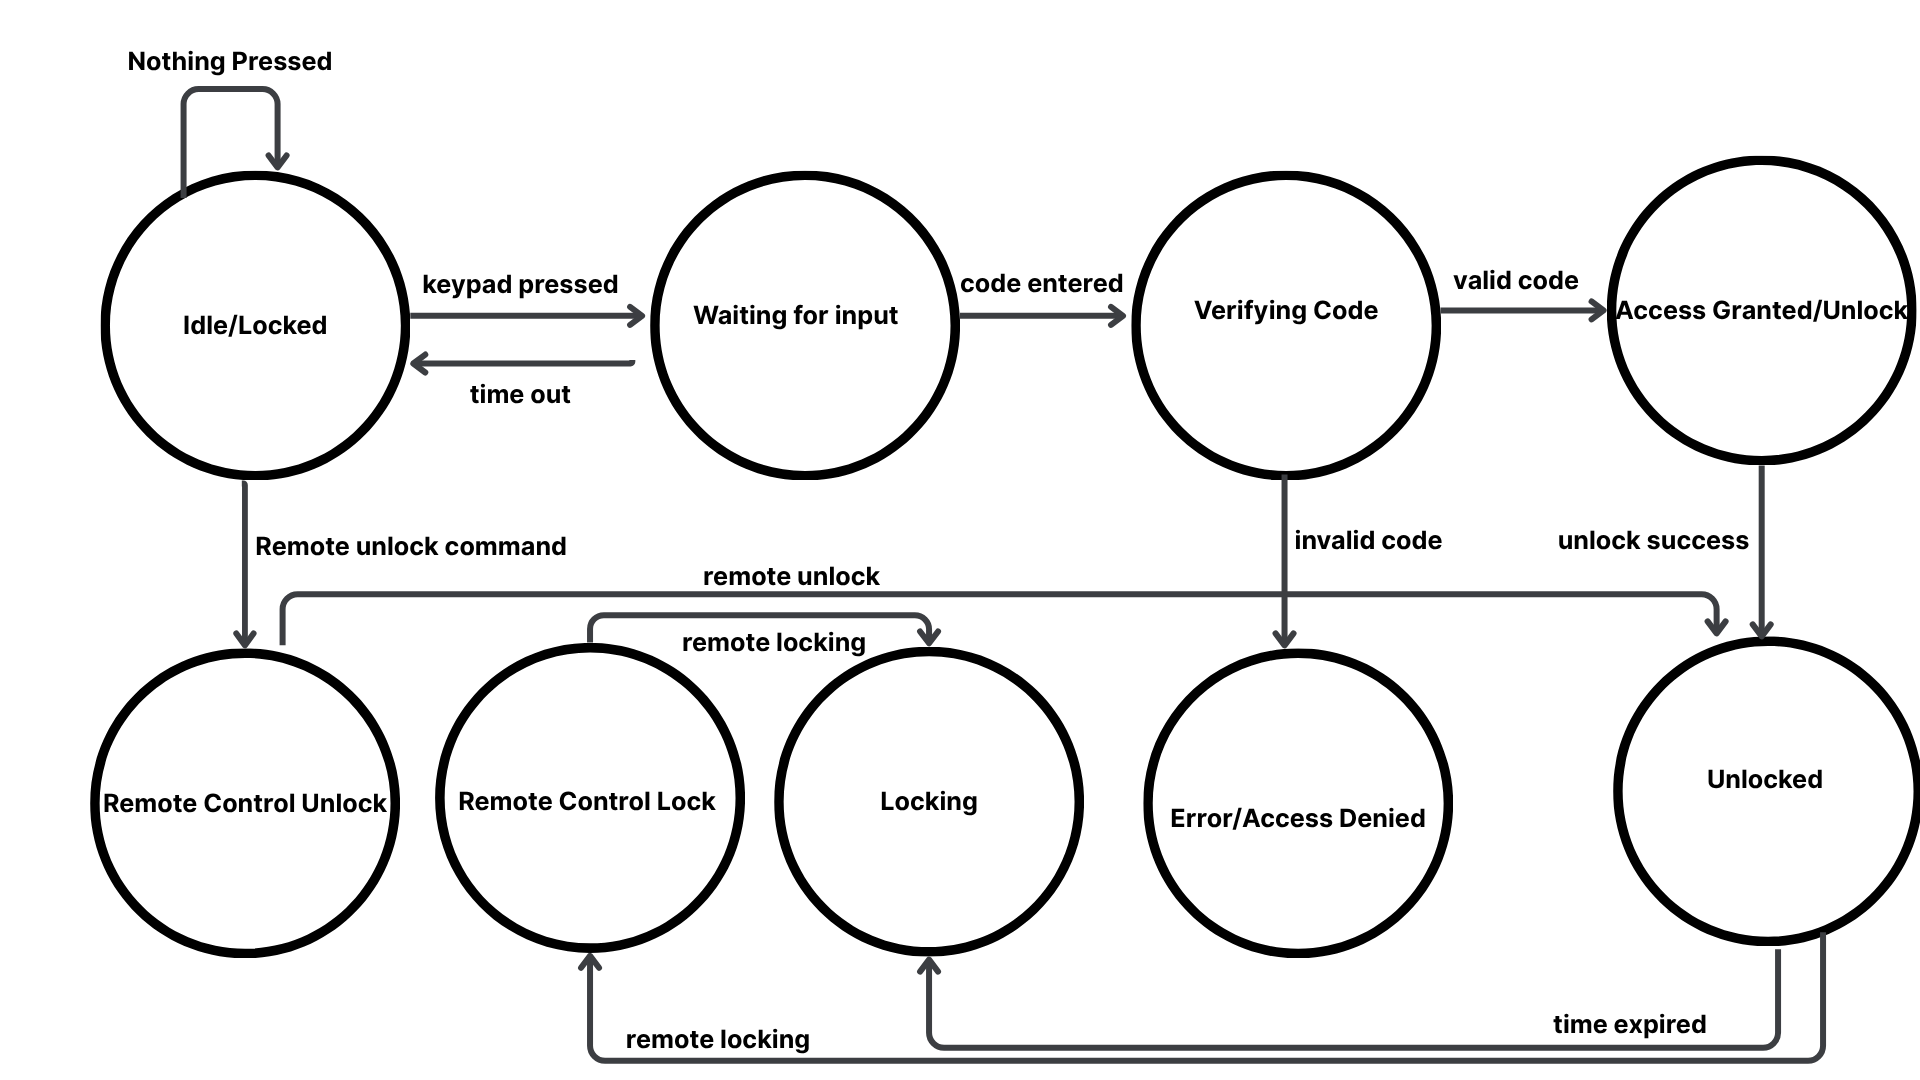
\includegraphics[width=0.80\textwidth]{img/stateTransitionDiagram.png}
    \caption{State Machine Diagram}
    \label{fig:stateTransitionDiagram}
\end{figure}

The system starts in the Idle/Locked state, where it remains until user interaction is detected. When a key is pressed on the keypad, the system transitions to the Waiting for Input state, where it captures the full access code. After the user submits a code, the system enters the Verifying Code state. At this point, the input is checked either locally or through server communication. If the code is valid, the system proceeds to the Access Granted / Unlocking state, where the solenoid is activated to unlock the door. Once unlocked, the system moves to the Unlocked state and remains there for a set duration to allow entry. After the timeout period, the system transitions to the Locking state, re-engaging the solenoid to secure the door, and finally returns to Idle/Locked. If the entered code is invalid, the system transitions to the Error / Access Denied state, providing feedback to the user (e.g., a buzzer or LED alert), before returning to Idle/Locked after a short delay. The system also supports remote interactions. A command from the mobile app can transition the system from Idle/Locked to Remote Control Unlocking, and from Unlocked to Remote Control Locking. These remote actions follow similar unlock and lock procedures as local interactions.

\subsection{Technology}
For our hardware components, we used the ESP32-C3 microcontroller, programmed in C++ using the Arduino IDE. To support our development, we integrated several key libraries: Firebase Client by Mobizt, ArduinoJson by Benoit Blanchon, WiFiManager by tzapu, and Keypad by Mark Stanley and Alexander Brevig. These libraries enabled reliable communication with our Firebase server, interfacing with the keypad for user input, and creating a Wi-Fi access point for initial smart lock configuration. 

As for the smartphone app, we used Swift with Xcode for development. This means that our application currently builds natively for iOS devices only, such as iPhones and iPads. The app allows users to unlock and lock the smart lock remotely, receive battery and connectivity status notifications, and manage temporary PIN codes.

While our current version supports iOS exclusively, we plan to explore cross-platform solutions such as Flutter or React Native in the future to make the app available on Android devices as well. This would broaden accessibility and improve compatibility for a wider range of users.

\subsection{Simulation}

To better understand the performance, reliability, and longevity of our smart lock system, we developed several system-level models: power consumption, timing responsiveness, and brute-force protection.

\textbf{Power Model:}  
We modeled the average power usage of the system based on both datasheet specifications and realistic use scenarios. In our optimized configuration, the ESP32-C3 remains in deep sleep mode (10~\textmu A) and only wakes on external interrupts (e.g., keypad input). During operation, the ESP32 briefly activates Wi-Fi and the solenoid for unlocking.

\begin{itemize}
    \item \textbf{Deep sleep:} 10~\textmu A for ~24 hours/day minus active time
    \item \textbf{Active mode:} 80~mA for 10 seconds per unlock (10 uses/day)
    \item \textbf{Solenoid:} 500~mA for 0.5 seconds per unlock
\end{itemize}

The total energy used per day is estimated as:
\[
\text{ESP32 (sleep)} \approx 0.0666~\text{mAh}, \quad
\text{ESP32 (active)} \approx 2.22~\text{mAh}, \quad
\text{Solenoid} \approx 0.694~\text{mAh}
\]
\[
P_{\text{daily}} \approx 2.98~\text{mAh/day}
\]

With a 3.7V 18650 Li-ion battery rated at 3,000~mAh, the expected runtime is:
\[
\text{Battery Life} = \frac{3,000~\text{mAh}}{2.98~\text{mAh/day}} \approx 1,007~\text{days} \approx \boxed{2.75~\text{years}}
\]

Factoring in losses due to regulators, temperature variation, and battery aging, a conservative real-world estimate is \textbf{1.5 to 2 years} of battery life per charge.

\textbf{Timing Model:}  
We modeled the response time from keypad input to unlocking to ensure a smooth user experience. Based on observed behavior and testing, the total average time is approximately 1.5 seconds:
\begin{itemize}
    \item Keypad entry: ~0.5 seconds
    \item Code verification (local/remote): ~0.3 seconds
    \item Solenoid activation and unlock: ~0.7 seconds
\end{itemize}

This timing model confirmed that our system remains responsive while conserving power.

\textbf{Security Model:}  
To mitigate brute-force attempts, we modeled the security of a 4-digit PIN system, which has 10,000 possible combinations. We implemented a lockout mechanism:
\begin{itemize}
    \item Maximum of 3 failed attempts before temporary lockout
    \item Lockout duration: 30 seconds
    \item Lockout resets after inactivity or power cycle
\end{itemize}

This simple model helps protect against unauthorized access while balancing usability.

These models helped guide hardware component choices (such as low-power microcontrollers and solenoid driver circuits), define software timing thresholds, and enforce robust security policies in our firmware design.

